%\documentclass[10pt,conference]{IEEEtran}
%\documentclass[9pt,conference]{sig-alternate}
%\documentclass[9pt,conference]{sig-alternate}
%\documentclass[10pt,print,letterpaper,nocopyrightspace]{sigplan-proc-varsize}
\documentclass[10pt,print,letterpaper]{sigplan-proc-varsize}

\usepackage{amsmath,epsfig}
\usepackage{url}
\usepackage{xspace}
\usepackage{colortbl}
\usepackage{subfigure}
\usepackage{dsfont}
\usepackage{boxedminipage}
\ifx\pdfoutput\undefined
\usepackage[hypertex]{hyperref}
\else
\usepackage[pdftex,hypertexnames=false]{hyperref}
\fi

\usepackage{amssymb}
\usepackage{wasysym}
\usepackage[left=2.54cm,top=2.54cm,right=2.54cm,bottom=2.54cm,nohead,nofoot]{geometry}



\DeclareMathOperator*{\argmax}{argmax}
%\usepackage{times}

\def\ucb{$^{\dagger}$}
\def\stanford{$^{\ddagger}$}
\def\arch{$^{\star}$}

\newcommand{\kb}{kB}
\newcommand{\rene}{Ren{\'e}\xspace}
\newcommand{\reneii}{Ren{\'e}2\xspace}
\newcommand{\wec}{WeC\xspace}
\newcommand{\mica}{Mica\xspace}
\newcommand{\micaii}{Mica2\xspace}
\newcommand{\micaz}{MicaZ\xspace}
\newcommand{\micadot}{Mica2Dot\xspace}
\newcommand{\iic}{I$^2$C\xspace}
\newcommand{\uA}{$\mu$A\xspace}
\newcommand{\dotmote}{Dot\xspace}
\newcommand{\mhz}{MHz\xspace}
\newcommand{\ghz}{GHz\xspace}
\newcommand{\kbps}{kbps\xspace}
\newcommand{\dsn}{DSN\xspace}
\newcommand{\io}{I/O\xspace}
\newcommand{\telos}{Telos\xspace}

\newcommand{\T}{\mathds{T}}
\newcommand{\XXXnote}[1]{{\bf\color{red} XXX: #1}}


\begin{document}

%\conferenceinfo{Sensys'08,} {November 5--7, 2008, Raleigh, NC, USA.}  
%\CopyrightYear{2008} 
%\crdata{978-1-60558-096-8/08/09} 

\title{Dissertation Notes:\\StreamFS and everything that comes out of it.}
%\numberofauthors{1} 
%\author{\alignauthor Stephen Dawson-Haggerty, Jorge Ortiz, Xiaofan Jiang and David Culler\\
%\affaddr{Computer Science Division}\\
%\affaddr{University of California, Berkeley} \\ 
%\affaddr{Berkeley, California 94720} \\
%\email{\{stevedh,jortiz,xjiang,culler\}@cs.berkeley.edu}
%} 


%\subtitle{Paper \# Insert Reg Number Here}

%\title{Alternate {\ttlit ACM} SIG Proceedings Paper in LaTeX
%Format\titlenote{(Produces the permission block, and
%copyright information). For use with
%SIG-ALTERNATE.CLS. Supported by ACM.}}
%\subtitle{[Extended Abstract]
%\titlenote{A full version of this paper is available as
%\textit{Author's Guide to Preparing ACM SIG Proceedings Using
%\LaTeX$2_\epsilon$\ and BibTeX} at
%\texttt{www.acm.org/eaddress.htm}}}
%
% You need the command \numberofauthors to handle the 'placement
% and alignment' of the authors beneath the title.
%
% For aesthetic reasons, we recommend 'three authors at a time'
% i.e. three 'name/affiliation blocks' be placed beneath the title.
%
% NOTE: You are NOT restricted in how many 'rows' of
% "name/affiliations" may appear. We just ask that you restrict
% the number of 'columns' to three.
%
% Because of the available 'opening page real-estate'
% we ask you to refrain from putting more than six authors
% (two rows with three columns) beneath the article title.
% More than six makes the first-page appear very cluttered indeed.
%
% Use the \alignauthor commands to handle the names
% and affiliations for an 'aesthetic maximum' of six authors.
% Add names, affiliations, addresses for
% the seventh etc. author(s) as the argument for the
% \additionalauthors command.
% These 'additional authors' will be output/set for you
% without further effort on your part as the last section in
% the body of your article BEFORE References or any Appendices.

\numberofauthors{2} %  in this sample file, there are a *total*
% of EIGHT authors. SIX appear on the 'first-page' (for formatting
% reasons) and the remaining two appear in the \additionalauthors section.
%
\author{
% You can go ahead and credit any number of authors here,
% e.g. one 'row of three' or two rows (consisting of one row of three
% and a second row of one, two or three).
%
% The command \alignauthor (no curly braces needed) should
% precede each author name, affiliation/snail-mail address and
% e-mail address. Additionally, tag each line of
% affiliation/address with \affaddr, and tag the
% e-mail address with \email.
%
% 1st. author
\alignauthor
%Prabal Dutta\\
%       \affaddr{Computer Science Division}\\
%       \affaddr{Univ. of California, Berkeley}\\
%       \affaddr{Berkeley, CA 94720}\\
%       \email{prabal@cs.berkeley.edu}
% 2nd. author
%\alignauthor
%David Culler\\
%       \affaddr{Computer Science Division}\\
%       \affaddr{Univ. of California, Berkeley}\\
%       \affaddr{Berkeley, CA 94720}\\
%       \email{culler@cs.berkeley.edu}
% 3rd. author
%\alignauthor
%Scott Shenker\\
%       \affaddr{Computer Science Division}\\
%       \affaddr{Univ. of California, Berkeley}\\
%       \affaddr{Berkeley, CA 94720}\\
%       \email{shenker@cs.berkeley.edu}
%}
Jorge Ortiz\\
       %\affaddr{Department}\\
	\affaddr{Computer Science Division}\\
       \affaddr{University of California, Berkeley}\\
       %\affaddr{City, State Zip}\\
       \email{jortiz@cs.berkeley.edu}
}


\maketitle

%\date{14 April 2007}
%\maketitle

\begin{abstract}
Despite the growing impact of climate change and energy prices, 
per-capita energy consumption is rising. Part of the problem is visibility. We do not 
have scalable means of observing our energy consumption patterns and determining how to optimize and reduce our
consumption.
Mobile smartphones present a unique opportunity to enable an energy view on the physical world. 
They can bridge the physical world, information infrastructure, and people
through a rich set of sensors, ubiquitous connectivity, and highly personal user interface. 
With QR codes as cheap tags on items and places in the physical world, the
camera becomes a portable scanner in your pocket, in addition to its
traditional functions.  We explore this
unique triple point
and re-examine classical problems of context and consistency management in mobile
systems.  We also examine this combination as it pertains to energy management of physical
devices.  In doing so, we are re-introduced to problems of apportionment and aggregation of sensor data,
except with a continuously changing set of constituents.  We describe our solution in a technique
called \emph{dynamic aggregation} that maintains moving aggregates as the
set of data sources changes over time.  We deployed our system in a 
141,000 square-foot building, tagging 351 items over 139 room across 7 floors.

% When combined with QR codes, the on-board camera provides us with a portable scanner

% The camera,
% when combined with QR codes, gives us a portable scanner and convenient mechanism for tying these world together. 
% In this paper, we describe our system and deployment experience for a mobile phone application the provides 
% user-centric energy-view of the physical world. We describe the challenges, specifically dealing with mobility, 
% and how we address them in a set of three separate applications: an energy auditing application, a 
% device energy scanner, and a personal energy counter. We also introduce a technique called \emph{dynamic aggregation}
% which allows us to seamlessly track the constituents of aggregated energy calculations, as they move from one 
% location to another.

% Despite the recent impact of global warming and a steady increase in energy prices, 
% per-capita energy consumption is rising. Part of the problem is about visibility. We simply do not 
% have any good ways of seeing how we consume energy, and therefore, how to optimize and reduce it. 
\end{abstract}

% A category with the (minimum) three required fields
%\category{B.0}{Hardware}{General}
%\category{B.4}{Hardware}{Input/Output \& Data Communication}

%\terms{Design, Implementation, Performance, Experimentation}

%\keywords{Churn, Link, Routing, Wireless, Sensor Network, Mote}

%\newpage

\section{Design Motivation}
Our system is designed for a class of sensor deployments for distributed monitoring applications where the 
number of sensors is large and each sensor's data rate is on the order of seconds to minutes.  The motivating
scenario is a building monitoring system that monitors health of HVAC system components, plug-load power draw, 
lighting system power-draw, temperature sensors, pressure sensors, and other physical processes and items
within the building.  Although the individual data rates are low, the aggregate data rates per deployment
can be quite large.  For example, a typical 5-10 story building can easily produce at rates that match and exceed high-quality
streaming video rates (i.e. 700-1200 Kbps).  StreamFS uses a pub-sub architecture and generalizes the pub-sub
model to support real-time stream data processing that produce derivative streams as new data sources.  This can easily
multiply the amount of data being stored and/or delivered subscribers.

StreamFS organizes \emph{physical data} from \emph{real-world physical objects} whose relationship
is \emph{as} important as the data they produce.  The relationship informs our queries and motivates our decision to expose
these relationships, explicitly, through naming.  Although we're fundamentally building our interface on top of a relational
data model, the decision to use a hierarchical namespace with symbolic links to expose the underlying
entity-relationship graph is useful for managing physical data from the real-world.  With the relational model
you may lose important semantic information information about the real-world in return for a high degree
of data independence~\cite{Chen76theentity-relationship}.  Our system is more concerned with capturing
entities and relationships which exist in the real world and our minds as well as information structure (organization
of information in which entities and relationships are represented by data) -- we use an entity-relationship
data model~\cite{Chen76theentity-relationship}.


The data is timeseries in nature, and since it's fundamentally related to readings taken in physical space, 
the associated metadata must be tightly coupled with each data stream.  The metadata
describes the units, calibration parameters, placement and other important stream-context information.  
Metadata should be treated as a first-class citizen in the system.  Such treatment
is typical in fields in the natural sciences, such as environmental and climate science, where the metadata sets the framework
for in.  Strict guidelines are given for recording and managing metadata~\cite{meta_climate}.  For the class
of applications we are designing for, such concerns are just as relevant and metadata management must be done with
great care.  For example, temperature measurements taken in various locations -- a room, a hot or cold water pipe, an air vent -- 
and in order to interpret the measurement, we need the units of measurement, the location of the sensor, and calibration parameters
(if we are getting raw readings that need to be converted to measurement values).

In addition, we must track the deployment as it evolves.  Changes in metadata change the interpretation-context of the associated data stream.  
For example, as a sensor gets older it goes through natural wear and tear which change the calibration coefficients.  When such 
coefficients are updated, the associated data must be coupled with the newly reported data.   Also, some sensors are mobile and move from location 
to location.  We have designed various mechanisms for handling deployment evolution and discuss these in section~\ref{sec:evolution}.

\subsection{Location information}
We wish to record and keep track of the placement of sensors throughout a space.  One method for recording spatial information
is to include geo-spatial coordinates for each sensor.  However, geospatial coordinates do not capture more relevant information
about what is being measured.  In a building, placement is more abstractly defined as the system or space in which the sensor
is placed, not the specific coordinates of placement.  Although a coordinate system could also be useful, system or space association
is more relevant in interpreting sensor readings.

In addition, geospatial coordinates are difficult to assign or determine in some locations -- particularly indoors due
to weak signals, fading, and multipath~\cite{indoorGPS}.  One could argue for the use of other infrastructure for determining coordinates
in such a setting, however, the challenges remain~\cite{multipath, cricket, wifiindoors}.  Still, referring to sensors based on placement
(with semantics ascribed by the user) is more important than determining the exact location.  Our system takes the approach of
describing placement through naming.  Our naming mechanism is simple and flexible enough to allow for arbitrary names
with ascribing meaning to the naming convention.  We leave interpretation semantics to the application.

\subsection{Naming}
Names should be human readable and interpretable, similar to DNS.  In buildings, sensors are referred to by the system or space
associated with the point of measurement.  Our approach was to use a hierarchical naming scheme, similar to a Unix filesystem.  
As explained in ~\cite{seltzerHierarchy},
hierarchy  restricts the user to retrieve their data according to how that piece of data is named. The full pathname conflates naming and access.
Although this can be limiting for data in a traditional sense, this restriction serves a very useful role in naming and retrieving data for
the building application example and deployments like it.  We illustrate this with an example in building sensor deployments.

Suppose there's a sensor on the first floor in room 100 in Soda Hall.  If we have different deployments, we can set the hierarchical
structure to have a path as follows `{\tt /buildings/soda/01/100/tempSensor}' that walks us down from the `{\tt /buildings}' which can represent
that set of buildings in our multi-deployment all the way from the building to the floor and finally the room where the sensor is placed.
It's natural to organize the data this way and useful from a human-readable perspective to immediate extract the context where the sensor
is based entirely on the access-path for that sensor.  This naming convention does not entirely cover all medata but it
simplifies access to relevant information.

%Multi-homing/naming and symbolic links
The experienced reader may have noticed in a building a sensor that drives a system may also sit in a space.  A sensor can be 
referred to through it's association with the system or its association with a space.  This observation implies the need for supporting 
multiple names.  We support multiple names through the use of symbolic links, similar to symlinks used in typical filesystems.
For example, if the {\tt tempSensor} is attached to a  variable air volume (VAV) component in the heating, ventilation and air conditioning
(HVAC) system; in other words, the temperature sensor drives the heating/cooling sub-system for that room.  Another name
for the same sensor is `{\tt /buildings/hvac/ventilation/vav/tempSensor}'.  To assure that both names refer to the same object we differentiate
between \emph{hardlinks} and \emph{symlinks} and either we make one of the two paths point to the hardlink or make both names symlinks
and create a hardlink with a different name that both paths point to.  In the mobile context, the latter approach is useful.  The object
reference remains static while the symlink references to the object change as the object moves from place to place.

\subsubsection{Additional metadata}
Naming does not capture all the metadata, so we included object/node annotations: user-defined properties that are attached to each object.
We support search by property values.   Geospatial, type, or other information can included in the annotation for the object.  Annotations are
flexible enough to allow for a wide range of application semantics.  For example, our building monitoring application defines a set of node
\emph{types} to represent different components in the HVAC sub-systems, electrical load tree, and zones inside the building.  More
details can be found at~\cite{buildingschemas}.

\subsection{Time and deployment evolution}
\label{sec:evolution}
Long-term deployments naturally evolve over time.  There are changes to the deployment settings and changes to sensors.  Sensors are
replaced, removed, and added.  The space being monitored expands or morphs.  Meter upgrades join new facts about the sensor(s)
with the sensor that replaced it.  As a concrete example, lets return to the building sensor deployment setting.  Buildings are often up for decades. 
During this time period, rooms are added and broken sensors are replaced.  If the temperature sensor in a room breaks it needs to be 
fixed or replaced.  Both involve certain new information to be recorded about the deployment, such as updates calibration parameters.  Although
the logical sensor-access name is unchanged, the physical object the name references has changed and such changes are important.

At a more infrequent rate, there may be changes to the physical structure of the building.  Two rooms may be combined into one.  An extra floor
may be added to accommodate more people or new building functions.  Such changes usually require changes to the underlying climate and
electrical systems.  New ducts and vents are added into the new spaces, expanding the reach of the current HVAC system.  A new, independent
HVAC system may be added altogether.  The electrical load tree must accommodate the new load, which requires additions to the underlying
structure of the electrical load tree.

These are impact the context in which measurements are being collected.  Without mechanisms to accurately track and account for
such changes, analysis about the behavior and consumption with respect to stale information will lead to gross miscalculations that get worse and worse
over time.

\subsubsection{Timeseries data, naming, metadata}
The data collected from deployments is fundamentally timeseries in nature.  However, physical data cannot be interpreted without its associated context.
Such context information is recorded in the metadata for each sensor stream.  As described in the previous sections, we partition the metadata into two
pieces.  The first piece captures placement information through naming while the second piece captures everything else.  In particular, the latter piece
should be used to record calibration information for the readings being collected.  The data and associated metadata are tightly coupled and we
must design mechanisms to maintain the integrity of this relationship through time.  Changes in placement, as recorded by the naming structure, are 
hereafter referred to as placement context while change in calibration or other descriptive information is hereafter referred to as descriptive or 
measurement context (both will be used interchangeably).

Timeseries data, placement context, and measurement context are bound through time.  For example, imagine a temperature sensor in a room sending periodic
temperature readings.  Upon installation, the temperature sensor is named with respect to its placement in the room, (i.e. {\tt /room/tempsensor01}).
With the newly created reference we record calibration information associated with the reference.  At some point in the future, the temperature sensor
is replaced.  We wish to keep the logical reference to the sensor, so we keep the name reference to same, however, the new sensor has different calibration
parameter that override the old ones.  In calculating, the average temperature of the room over that timespan, we need to re-structure the placement and measurement context in order to make an accurate assessment of the average temperature.  Using latest calibration parameters would give false readings
for the original sensor.  Moreover, if at some point later, we install a completely new temperature sensor model and delete the current reference altogether,
we still want to ``remember'' that we had the old model in the past in order to calculate the average temperature with the old readings.

%Use a object id to couple the timeline udpates.

Both scenarios require the coupling of separate timelines.  Attached to each set of readings is the metadata that describes the context of
the data.  The metadata in StreamFS consists of the path(s) and properties associated with the object.  The state of this set uniquely identifies
an object and any changes to the set of path(s) or properties generates a new object identifier.  The object identifier (\emph{oid}) is 
unique 128-bit number.  The high-order 96 bits are unique to the object, while the remaining low-order 32 bits are the version number.  When a change
occurs to the metadata we increment the version portion of the identifier.  We also record the time when the change was made.  As the data is stored, 
the oid is attached to each inputted value.  This allows us to explicitly couple the metadata with the data.  The timestamps are used for
snapshot and rollback queries.


% Both scenarios require the ``stitching'' of separate, but related, timelines.  The timeseries data is naturally a set of readings recorded over time, the 
% placement context or naming structure is on another timeline, and the measurement context is on its own timeline.  As we go back in time, we first determine
% the existence of a temperature sensor in the room using the naming structure, we locate the point in time in which the measurement context was in effect,
% and we grab the data through that time interval and use the measurement context to calculate the correct readings.  We continue this process throughout the
% specificed query interval.  Finally, we take the calculated readings and compute the average.  The ``timeline-stitching'' (TLS) process is demonstrated
% in figure~\ref{fig:timestitch}.  Queries that require \emph{timeline-stitching} are called ``metadata timeseries queries'' or \emph{MTSQ}.


In section~\ref{sec:mtsq} we discuss the different types of MTSQ's, their relationship to traditional mechanisms used in temporal databases, and
the complexity and performance issues for storing timelines and executing TLS's for MTSQ's efficiently.  Dealing with MTSQ's over time intervals 
with many changes is the main challenge in running fast, efficient queries.  We have implemented a set of algorithms and caching technique that
allow MTSQ's to run with very little overhead, when compared to a tranditional timeseries query.  The average overhead is only {\tt X}\% in the average
case and no worse that {\tt Y}\% when compared to the standard timeseries query performance.  In addition, we show how MTSQ's help simplify the
tracking and subsequent accuracy of derivative historical calculations.


\subsection{Derivative streams}


\subsection{Mapping relationships explicitly}














\section{Metadata timeseries queries}
\label{sec:mtsq}
whataksndlkasndlkasn


\subsection{Objects and data}
%
% 	join by global object identifier (128 uuid: 96-bit object_id, 32-bit version sequence)
%
%	Create a lookup service (read INS paper for ideas) to lookup the object
%	It will probably involve something like the work in mobile IP, I3/Ocala, and INS
%
%	Example lookup syntax:
%		sfs://jortiz81.homelinux.com:8080::550e8400-e29b-41d4-a716-4466-554400CF


\subsection{Structural snapshot}

\subsubsection{Storage}

\subsubsection{Querying}

\section{Relationship to OLAP}
The main terms in OLAP consist of Dimensions, Measures, Hierarchies, and Grain.  Dimensions are the axes of aggregation.
For example, you may want to aggregate with respect to location, time, or type.  Measures are the units or category of
measurement that you're making for the data values assocaited with a dimension.  For example, cost is a type of measure,
so is revenus and quatity.  There are hierarchies in the data that dictate the relationship between the dimensions
and how that relationship influences the amount of derived data and computation that needs to be done to satisfy
these hierarchical aggregations.  The grain of the data is the lowest level of granularity.  Abstractly, the lowest grain
in OLAP is the actual transaction.  In the context of StreamFS, it's the raw stream coming in from a stream source.

In a typical OLAP setup, hierarchies do not change, dimenions do not change, grain does not change, measures do not change.
OLAP is perfect for industries with structured analytical accounting such as finance and accounting but less of a fit for
sales, operations, marketing, and R\&D.

% Keyword:  dimensional-relational model -- using the relationshal model (star, snowflake, constellation schemas)
% to logically construct the OLAP hypercube.

% It's extremely difficult, using the star schema in the OLAP hypercube approach, to add a dimension.  The main operations
% on the hypercube are privoting, roll-up, and sub-cube extraction.

What's different here is that the dimensions change -- measures have multiple coordinates at any point in time and the coordinates
change as a function of time, not just measures themselves.  Dimensional coordinates are expressed by tags, where the time dimension,
exists both for measures produced by stream objects and the tags themselves.  The tags are used to reconstructed the relational-DAG
between the dimensions and the objects at any point in time.

% Indexing will have to be addressed.  How do you set up the index structures to get comparable results	to traditional OLAP queries?

\begin{itemize}
\item Explain how are the tags used to handle dynamic dimensionality.
\item Explain how the tags are used to handle hierarchical relationships.
\item Explain how tags are used to support multi-dimenionality (multi-naming).
\item Explain how OLAP operations are performed using these naming approach.
	\begin{itemize}
	\item Rollup.
	\item Drill-down.
	\item Pivoting.
	\item Slice and Dice.
	\item time.
	\end{itemize}
\item Explain how the indexing is done to support these operations efficiently -- use each of the operations for demonstration.
\item Explain how timeseries queries account for dimensionality and hierarchical changes.
\end{itemize}


StreamFS is an analytical framework that provides streaming OLAP for operational processes with schema timeline consistency.
\begin{itemize}
\item streaming olap
\item changing dimensions
\item metadata timeline consistency management
\end{itemize}







% \section{Experience Lessons learned}
% \begin{enumerate}
% \item engagement is necessary
% \item we must capture all devices, meters, \emph{and} their inter-relationship
% \item we must capture some location and other information about each entity for accounting
% \end{enumerate}

% \section{Challenges: Automation}
% \begin{enumerate}
% \item mobility
% \item bind-dissociation/re-association
% \item energy apportionment/accounting
% \end{enumerate}

\section{Projected results}
\begin{enumerate}
\item audit results
\item energy usage take-aways
\item query time for a typical single-device/lookup query
\item query time for an aggregate query
\end{enumerate}

% \begin{figure}[htb!]
% \begin{center}
% 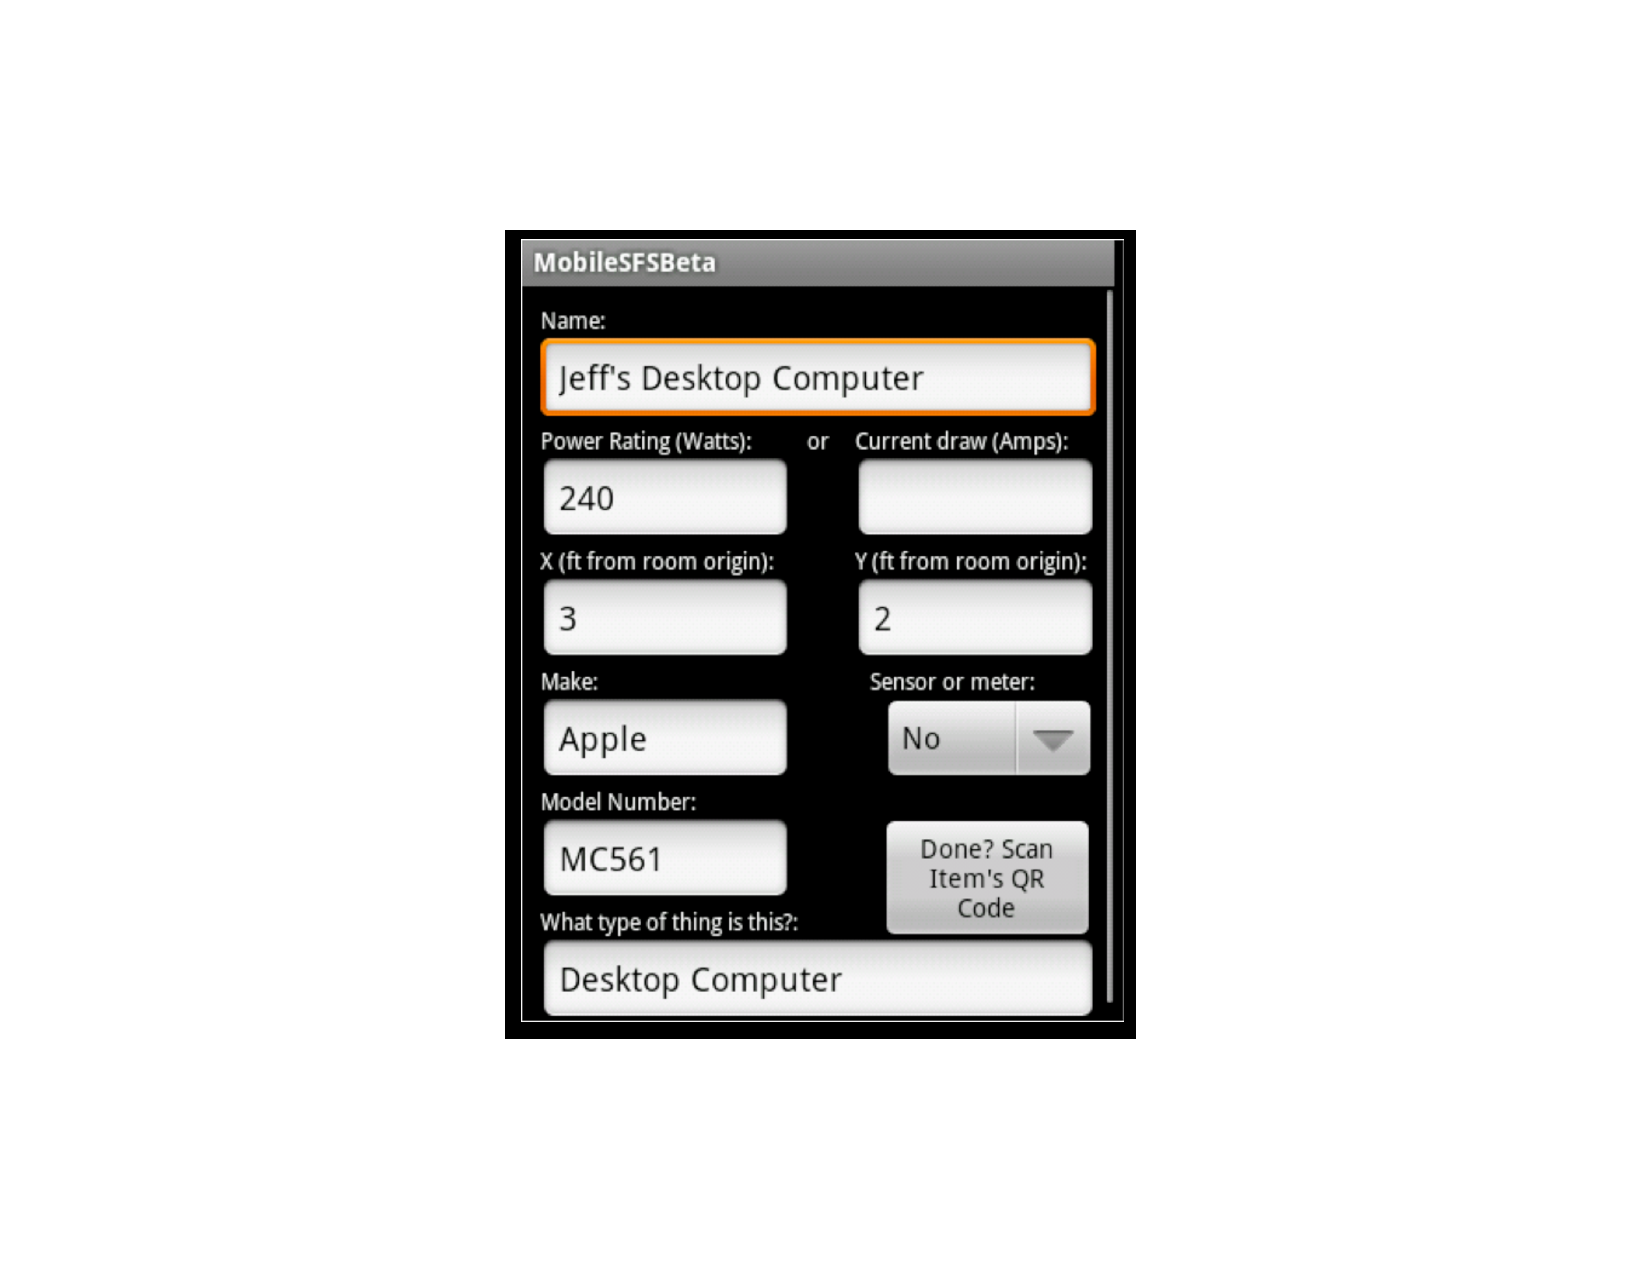
\includegraphics[width=0.8\columnwidth]{figs/screenshot01}
% \caption{The interface presented to the user for entering device and meter information.}
% \label{channelcomp}
% \end{center}
% \end{figure}



\section{Mobile SFS}
\label{sec:mobile}
The phone is the natural point of intersection between the user, the phyiscal world, and virtual services.\\

{\bf Goals}:
\begin{itemize}
\item Personalized energy attribution and tracking
\item Auto-aggregation techniques using stream correlation analysis \\
	\begin{itemize}
	\item identify stream correlations
	\item aggregate according to correlation threshold
	\item at user level, location level, total
	\item dealing with mobility (re-association and aggregation of streams) with dynamic subscriptions
	\end{itemize}
\end{itemize}

{\bf How do we know that the streams being aggregated are the right streams to aggregate?  What's the ground truth?}
Should we ask the user? (this becomes a user study)

The next approach skips this step altogether and establishes \emph{goodness} by comparing before/after aggregate consumption
data for the office.  Does the auto-aggregation help with this at all?

Is this about user engagement or is this about accuracy?  For a systems paper this really should be about accuracy
and should be compared against ground truth.  Ground-truth in this case is user behavior before and user behavior afterwards.


{\bf calibration might be an issue}

\begin{itemize}
\item Items that we were once used together that are no longer used together.
\item Energy consumption per user drops.
\item Cumulative energy consumption drops.
\end{itemize}

{\bf Accounts}:
\begin{itemize}
\item spaces
\item users \\
\end{itemize}

Users use their mobile phone to tag items they are actively using. \\

{\bf Tagging and registration mechanisms}:
\begin{itemize}
\item scan the qr code of the item you are currently using
\item if the item is a shared item, then it can be tagged by multiple users, and the energy can be split amongst all the users
	\begin{itemize}
	\item if a non-personal item is actively being used and nobody claims it, it is charged to all the users that we were in the same space
			as the item when the item became active.
	\item if a non-personal item is actively being used and nobody claims it and nobody was in the space when the item was turned on, it is charged
			to the space.
	\end{itemize}
\item if the item is a single-use item, it can only be used by a single user at time
\item if the item is a personal item, it can only belong to a single user and all energy is charged to that single user \\
\end{itemize}


{\bf Hypotheses}:

\begin{enumerate}
\item Personal energy attribution helps induce changes in behavior that lower energy consumption.
\item Personal energy attribution requires active user participation and engagement.
	\begin{itemize}
	\item Localization can be automated with indoor wifi; lowering participation overhead.
	\end{itemize}
\end{enumerate}



\subsection{Tracking steps}

\begin{enumerate}
\item Bootstrap
\item Tracking
\item Analysis
\item Visualization
\end{enumerate}


\subsubsection{Bootstrap}
The bootstrap phase is step where users become aware that there is energy information out there and it's the essential bootstrapping processes
of getting the user invovled in their energy attribution.  This step consists of:

\begin{enumerate}
\item Tagging items of everyday use with qr codes.
\item Binding meters and items.
\item Tag items as personal, shared, n-multi-shared
\end{enumerate}


All items should be tagged with qr codes.  This involves physically sticking a qr code onto the item, scanning it, and describing the item
that it is attached to.  This should be done for {\bf all items with a measurable energy footprint}, including lights, computers, appliances,
chargers, space heaters, etc.  -- miscenallenous eletrical loads.  A more advanced setup could include eletrical load information or HVAC 
component tagging, if visibility of total energy footprint is of interest.

Binding meters and items is a way of informing the system that the meter serves as an energy-consumption proxy for the item that the meter is
attached to.  This involves scanning both the meter and the item and creating their relationship explicitly.  This allows the application to query
the appropriate meter for historical consumption information when the user wishes to learn about the consumption of the item that is attached to that meter.
This model also assumes that meters are essentially free with respect to energy consumption.  Generally this assumption is not that far from reality.
For example, the ACme~\cite{acme} plugload meter draws on the order of several hundred milliwatts of power versus the tens to hundreds of watts being
consumed by the items it is typically measuring.

Tagging is the final, important step in the engagement phase.  This step requires that user scan items and essentially mark them as personal or shared.
This is used for analytical purposes and attribution.  You cannot determine which account the energy consumption of an item should be debited to without
ownership information.  Our application distinguishes between three types of sharing.  Personal items means that there is an owner relationship between
the item and its owner.  Any energy consumed by the item is attributed to the owner.  Shared items are charged to the user that last made use of the item.
If no user takes ownership of the item it is charged to every user of the system and each user is actively informed of the added charge (discussed in
section~\ref{sec:charge_alerts}).  Finally, the n-multi-shared items are items that can only be shared by N users at any one time.  This feature is essentially
sets an upperbound on the number of accounts that can be chared for the energy consumption of the device.

The cost of engagement is intially high but reduces over time.  The feature that we like best here is that the infrastructure captured through the engagement
step is beneficial for all users in the system and can be constructed iteratively.  The more users you have engaged, the faster the physical infrastructure
can be virtualized.

\subsubsection{Tracking}
%Scan you location/usage.

Tracking is the most active step in the attribution cycle.  This is where the user uses the application to record their location and energy consumption
information.  The infrastructure constructed in the \emph{bootstrap} step allows the user to scan their location and item being used.  For example, when the user walks into a building, she scans the qr code for the building to set their context.  As the user enters their office, they scan the qr code for the office.  Finally, 
before using any electrical device, the user scans it to register it's use.  Personal tags are most useful here, as they reduce this scanning step.
When the user is done using their item, they scan the item again to record that they are no longer using it.

This phase in the processes is the most tedious for the user and we think that more infrastructure and learning can be done to improve tracking.
To minimize interaction we offer mechanisms for grouping usage patterns.  For example, the user can decide to group items into an activity and 
combine streams for items that are associated with that activity.  For instance, each morning a graduate student comes to lab at the same time, 
turns on their PC or laptop, lamp, and prints out some papers.  The student pay group these streams into a single activity which alerts the application
to bin the energy consumed by the associated device to the account belonging to the user.

We also run correlation analysis in the background that looks to associate patterns of usage.  These may be presented to the user for corroboration
and ease the grouping processes.  We discuss its use in section~\ref{sec:correlation_analysis}.

% Analytical triggers

\subsubsection{Analysis}
Using traces generated by user activity, we track their energy usage through detailed accounting.  Our application combines energy consumption data
with contextual streaming data (i.e. location, usage information).  We perform aggregation in time, space, and category per user and group by activity
and location.  We also looks for trends in the data that indicate correlated usage patterns between items and users.  This allows us to ask
the user specific questions about grouping to make out analytics more accurate and reduce the burden imposed on the user during the tracking phase.
It also enables us to present the data to users about correlations amongst one another that could help them plan to use items more efficiently
from an energy perspective.  Details on our analysis is presented in~\ref{sec:analysis_results}.

\subsubsection{Visualization}
Finally, we looks for interesting ways of presenting real-time analytical data to users that could help them understand their own energy usage, as
well as the context of energy usage in their environment.  Our specific aim in this phase is to induce changes in behavior that cause the user to
make better use of their devices and reduce their overall energy consumption.  We demonstrate some of the visualization in section~\ref{sec:viz}
and the overall energy consumption before and after using the application in section~\ref{sec:energy_before_after}.


\section{Results}
This section will go start, first by talking about the overall energy consumption results.  For this, a baseline must be established, either
at the room-aggregate level or the individual user level.  The latter is simpler and is useful for comparing the effect of the system on invidual
energy consumption.  That's really the point of the system.






%\section{Related work}

%\begin{itemize}
% \item dashboard
% \item andrew's lightin control work
% \item Kamin's hvac control work
% \item BEMs
% \item sMAP stuff
%\item Buildsys 2010 work~\cite{hbci}
%\item distributed consistency management: COPS
%\item mobility: tracking things with RFID~\cite{rfid_gonz2006}
%\item mobility: tracking of people, wifi indoor localization
%\item entity-relationship graphs
%\item homeOS [microsoft]
%\item HP Cooltown~\cite{cooltown}
%\end{itemize}
Our work touches on several areas from smart home research to logistics.  In the building space, there has been
some interest in building various kinds of energy-related visual and control applications.
This work focuses on the object definition, tracking, and management component of the architecture proposed by 
Hsu et al.~\cite{hbci}.  Their work stratefied the set of challenges that one could potentially face if the application 
were deployed at scale.  Our
work, in constrast, bases its design rationale on a \emph{real deployment} that is taking place at scale in a building 
on our campus.  We focus on solving fundamental systems challenges in dealing with intermittent connectivity
and conflict resolution in tracking people and things over time.  We also focus on leveraging gestures to minimize
the cost of interaction for users, while maximizing the information we can attain about the state of the world.

% Tracking people/indoor localization
An important aspect of the Energy Lens is determining when people and things have moved.  This requires some form 
of indoor localization.  There's a large body of literature in the area of indoor localization with mobile phones ranging from 
using wifi~\cite{radar}, to sonar~\cite{cricket}, to ambient noise~\cite{abs}, and a combination of sensors on the 
phone~\cite{surroundsense, darwinphone}.  Dita~\cite{dita} uses acoustic localization of mobile phones and also uses the infrastructure 
to determine gestures in free-space that are classified into pre-defined control actions.  Each of these require relatively complex 
software and/or infrastrure.  
We take a radically different, simple approach.  We use cheap, easy to re/produce tags (QR codes), place them on things in the 
environment over incrementally and use the natural \emph{swiping gesture} that users make, when interacting with the Energy Lens 
application, to track when they have moved or when the objects around them have moved.  The working principal is to attain as much 
information from their gesture to determine when something/one has moved.  We discuss our heuristics in section~\ref{sec:swipes}.

% context-aware apps
ACE~\cite{ACE} uses various sensors on the phone to infer a user's context.  The context domain consists of a set of user activities
and semantic locations.  For example, if ACE can distinguish between {\tt Running, Driving, AtHome, or InOffice}.  ACE also infers 
the one from the others, so if the user is {\tt AtHome} then they are not {\tt InOffice}.  Energy Lens uses inference to determine
when a person or thing has moved.  Certain swipe combinations give us information about whether they moved and where they moved to or
whether an item moved and where it moved to.  The main difference is that we only infer context when a user is actively swiping, rather
than a continuous approach.  Pretching is a fundamental technique used in many domains.  However, the cost of a prefetch for mobile
application outways the benefits if the prefetched data is not useful.  Informed mobile pretching~\cite{IMP} uses cost-benefit analysis 
to determine when to prefetch content for the user.  In the Energy Lens context, we prefetch data based on their location swipes.
We also rely on pretching to anticipate loss of connectivity, not just to improve preformance.

% Tracking things
Logistic systems focus on the tracking of objects as the move through distribution sites to warehouses, stores, shelves,
and purchase.  Items are tracked through bar code or RFID readers.  However, the workload is very structured and well
defined.  The authors of~\cite{rfid_gonz2006} describe this structure and leverage it to minimize storage
requirements and optimize query-processing performance.  Energy Lens uses the QR codes as the tag and the phone as an active
reader.  As objects move, users scan those items to their new location.  However, objects may belong to one or
many people, they can be metered by multiple meters a day, and their history in the system
is on-going.  In contrast, a typical logistics workload has a start (distribution site) and end point (leaving the store
after a sale).  In our workload, relationship semantics are important; we need to know whether the meter is \emph{bound-to}
rather than simple \emph{attached-to} an item.  We discuss the difference later in the paper.
% In addition to traditional logistics-style queries -- \emph{What is the average time that it took coffee-makers to move from the 
% warehouse to the shelf and finally to the checkout counter in January of 2004?} -- energy-analytics requires queries to group
% partial traces from meter data by tracking what meters the item attached to over the specified time-frame.
% The Energy Lens system collects and manages this kind of information to enable such queries.
Furthermore, we take advatange of natural gestures the user makes with the phone while scanning QR codes to extract
information about the current location of the user or things.

% Tagging items, virtual services
The key idea in the HP Cooltown~\cite{bridgingphysical,cooltown} work is to web-enable `things' in the world, grouped-by
`place', and accessed by `people' via a standardized acquisition protocol (HTTP) and format (HTML, XML).  
Cooltown creates a web presence for things in the world either directly (embedded web server) or indirectly 
(URL-lookup tag) as a web page page that display the services it provides.  Many of the core concepts in Cooltown 
also show up in Energy Lens.  The main overlap is the use of tags in the world that contain a reference to a virtual 
resource, accessible via HTTP through
a network connection.  Cooltown, however, explicitly chooses not maintain a centralized relationship
graph, it leverages the decentralized, linking structure of the web to group associated web pages together.
Furthermore, things are assumed to not move.  People are the main mobile entities.  The kind of applications
we wish to support must track where things are and their specific inter-relationships.  We imposed a richer set of 
semantics on our, centrally maintained, relationship graph and use it to provide detailed energy information.


%\input{section1}
%\subsection{Results}

We test our hypothesis in this section by using EMD to remove low-frequency trends in the data
and run correlation calculation at overlapping IMF timescales.  We discover that EMD allows us
to find and compare high-frequency instrinsic behavior that is spatially correlated across
sensors.  We begin with a small set of three sensors (EHP, GHP, light) and expand our scope
to include all the sensors in the dataset.



\subsubsection{Initial analysis}
Lets consider the simple example of Section \ref{problem} where we would like to know if the EHP trace is correlated with the two other traces.
Recall that the correlation coefficients of the raw feeds was $0.7715$ and $0.6370$, corresponding to the light 
and GHP, respectively.
As stated in previous section this result is correct but not so meaningful, since most of the traces
display the same diurnal pattern.
Figure \ref{fig:emd} and Figure \ref{fig:emd2} show the EMD decomposition of the three traces.
For each trace, EMD has retrieved three IMFs that highlight the higher frequencies of the traces.

Figure~\ref{fig:emd} shows the normalized raw trace (top) and EMD output IMFs and residual as well as the 
correlation coefficients calculated on the IMFs for the EHP and
light traces.  The correlation coefficients are $0.43909$, $0.49344$ and $0.63469$ corresponding to the IMF1, 
IMF2, and IMF3, respectively.  Notice the high correlation between the high-frequency IMFs.
We know that the light and EHP serve the same room, and their high-frequency IMF correlation corroborates
our prior knowledge.
Figure~\ref{fig:emd2} shows a complementary result, for the EHP and GHP comparison.
The correlation coefficients for the EHP and GHP IMFs suggest that the two may be independent.  In fact, they
\emph{are} indepdent; they serve completely different rooms in the building!

EMD allows us to remove low-frequency trends that add noise to the original analysis.
By comparing IMFs, we see both intrisically correlated and \emph{uncorrelated} behavior.  In the next
section we expand our analysis and show the effectiveness of our methodology. 
% Although promising, these results must be validated across the rest of the
% dataset to confirm their significance.  


\subsubsection{Validation}
To validate the effectiveness of our approach, we analyze the same three-week time span for \emph{all} 674 
sensors deployed in the building.
For each trace $S$ we compute two scores: (1) the correlation coefficient between $S$ and the EHP trace
and (2) the average value of the IMF correlation coefficients.

\begin{figure}[tbh!]
\centering
 \subfloat[Raw traces correlation coefficients]{\label{fig:histo1}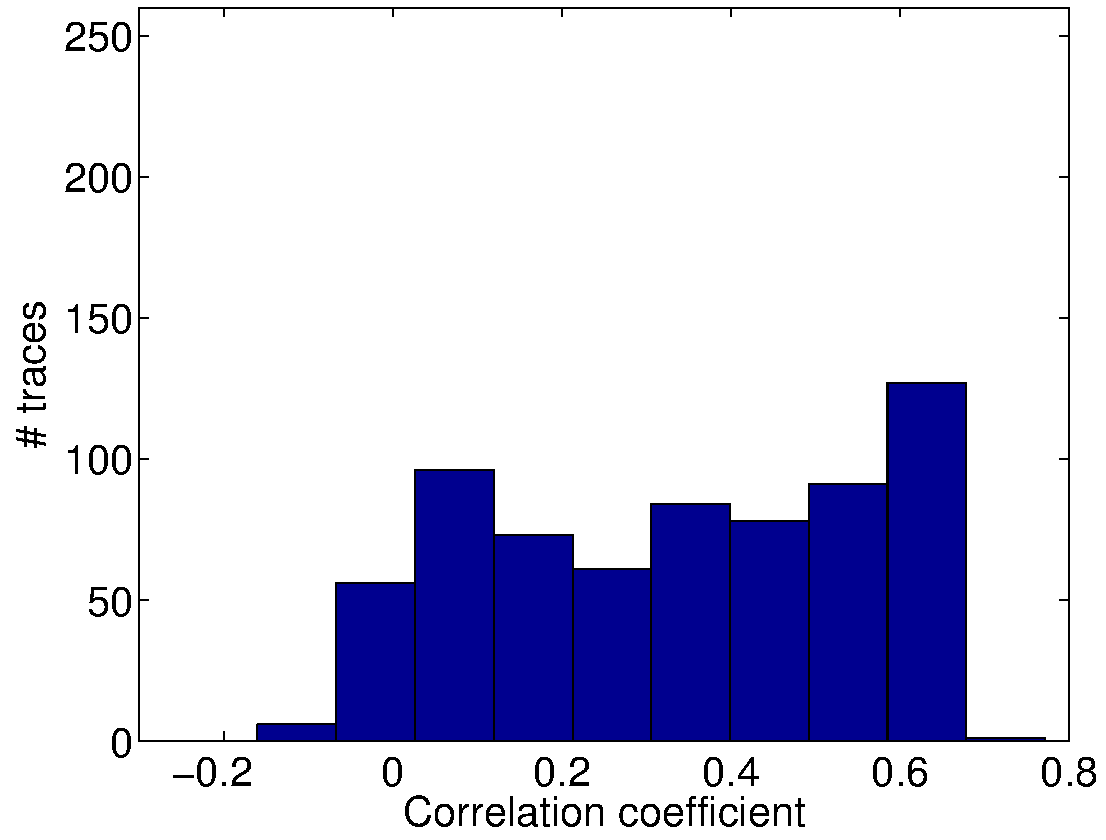
\includegraphics[width=.43\textwidth]{figs/allFloors_week1_week4_corr_abs-eps-converted-to}}
 \subfloat[Average IMFs correlation coefficients]{\label{fig:histo2}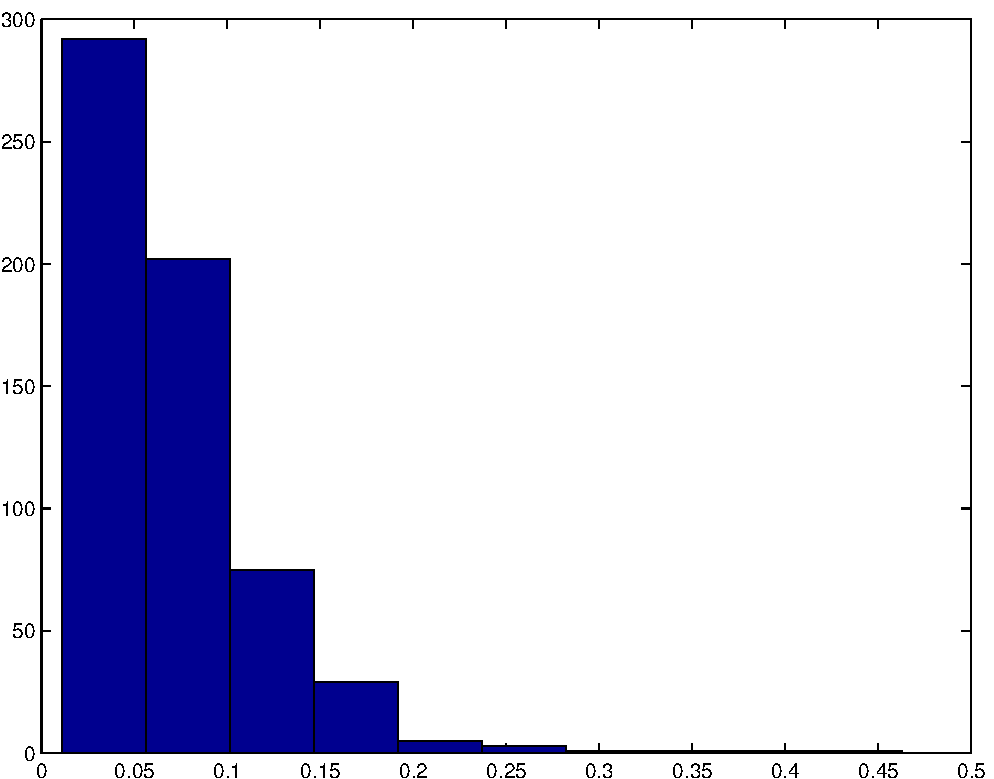
\includegraphics[width=.43\textwidth]{figs/allFloors_week1_week4_emd_abs-eps-converted-to}}
 \caption{Distribution of the correlation coefficients of the raw traces and correlation coefficients average of the corresponding IMFs using 3 weeks of data from 674 sensors.}
\label{fig:histo}
\end{figure}

\begin{figure}
\centering
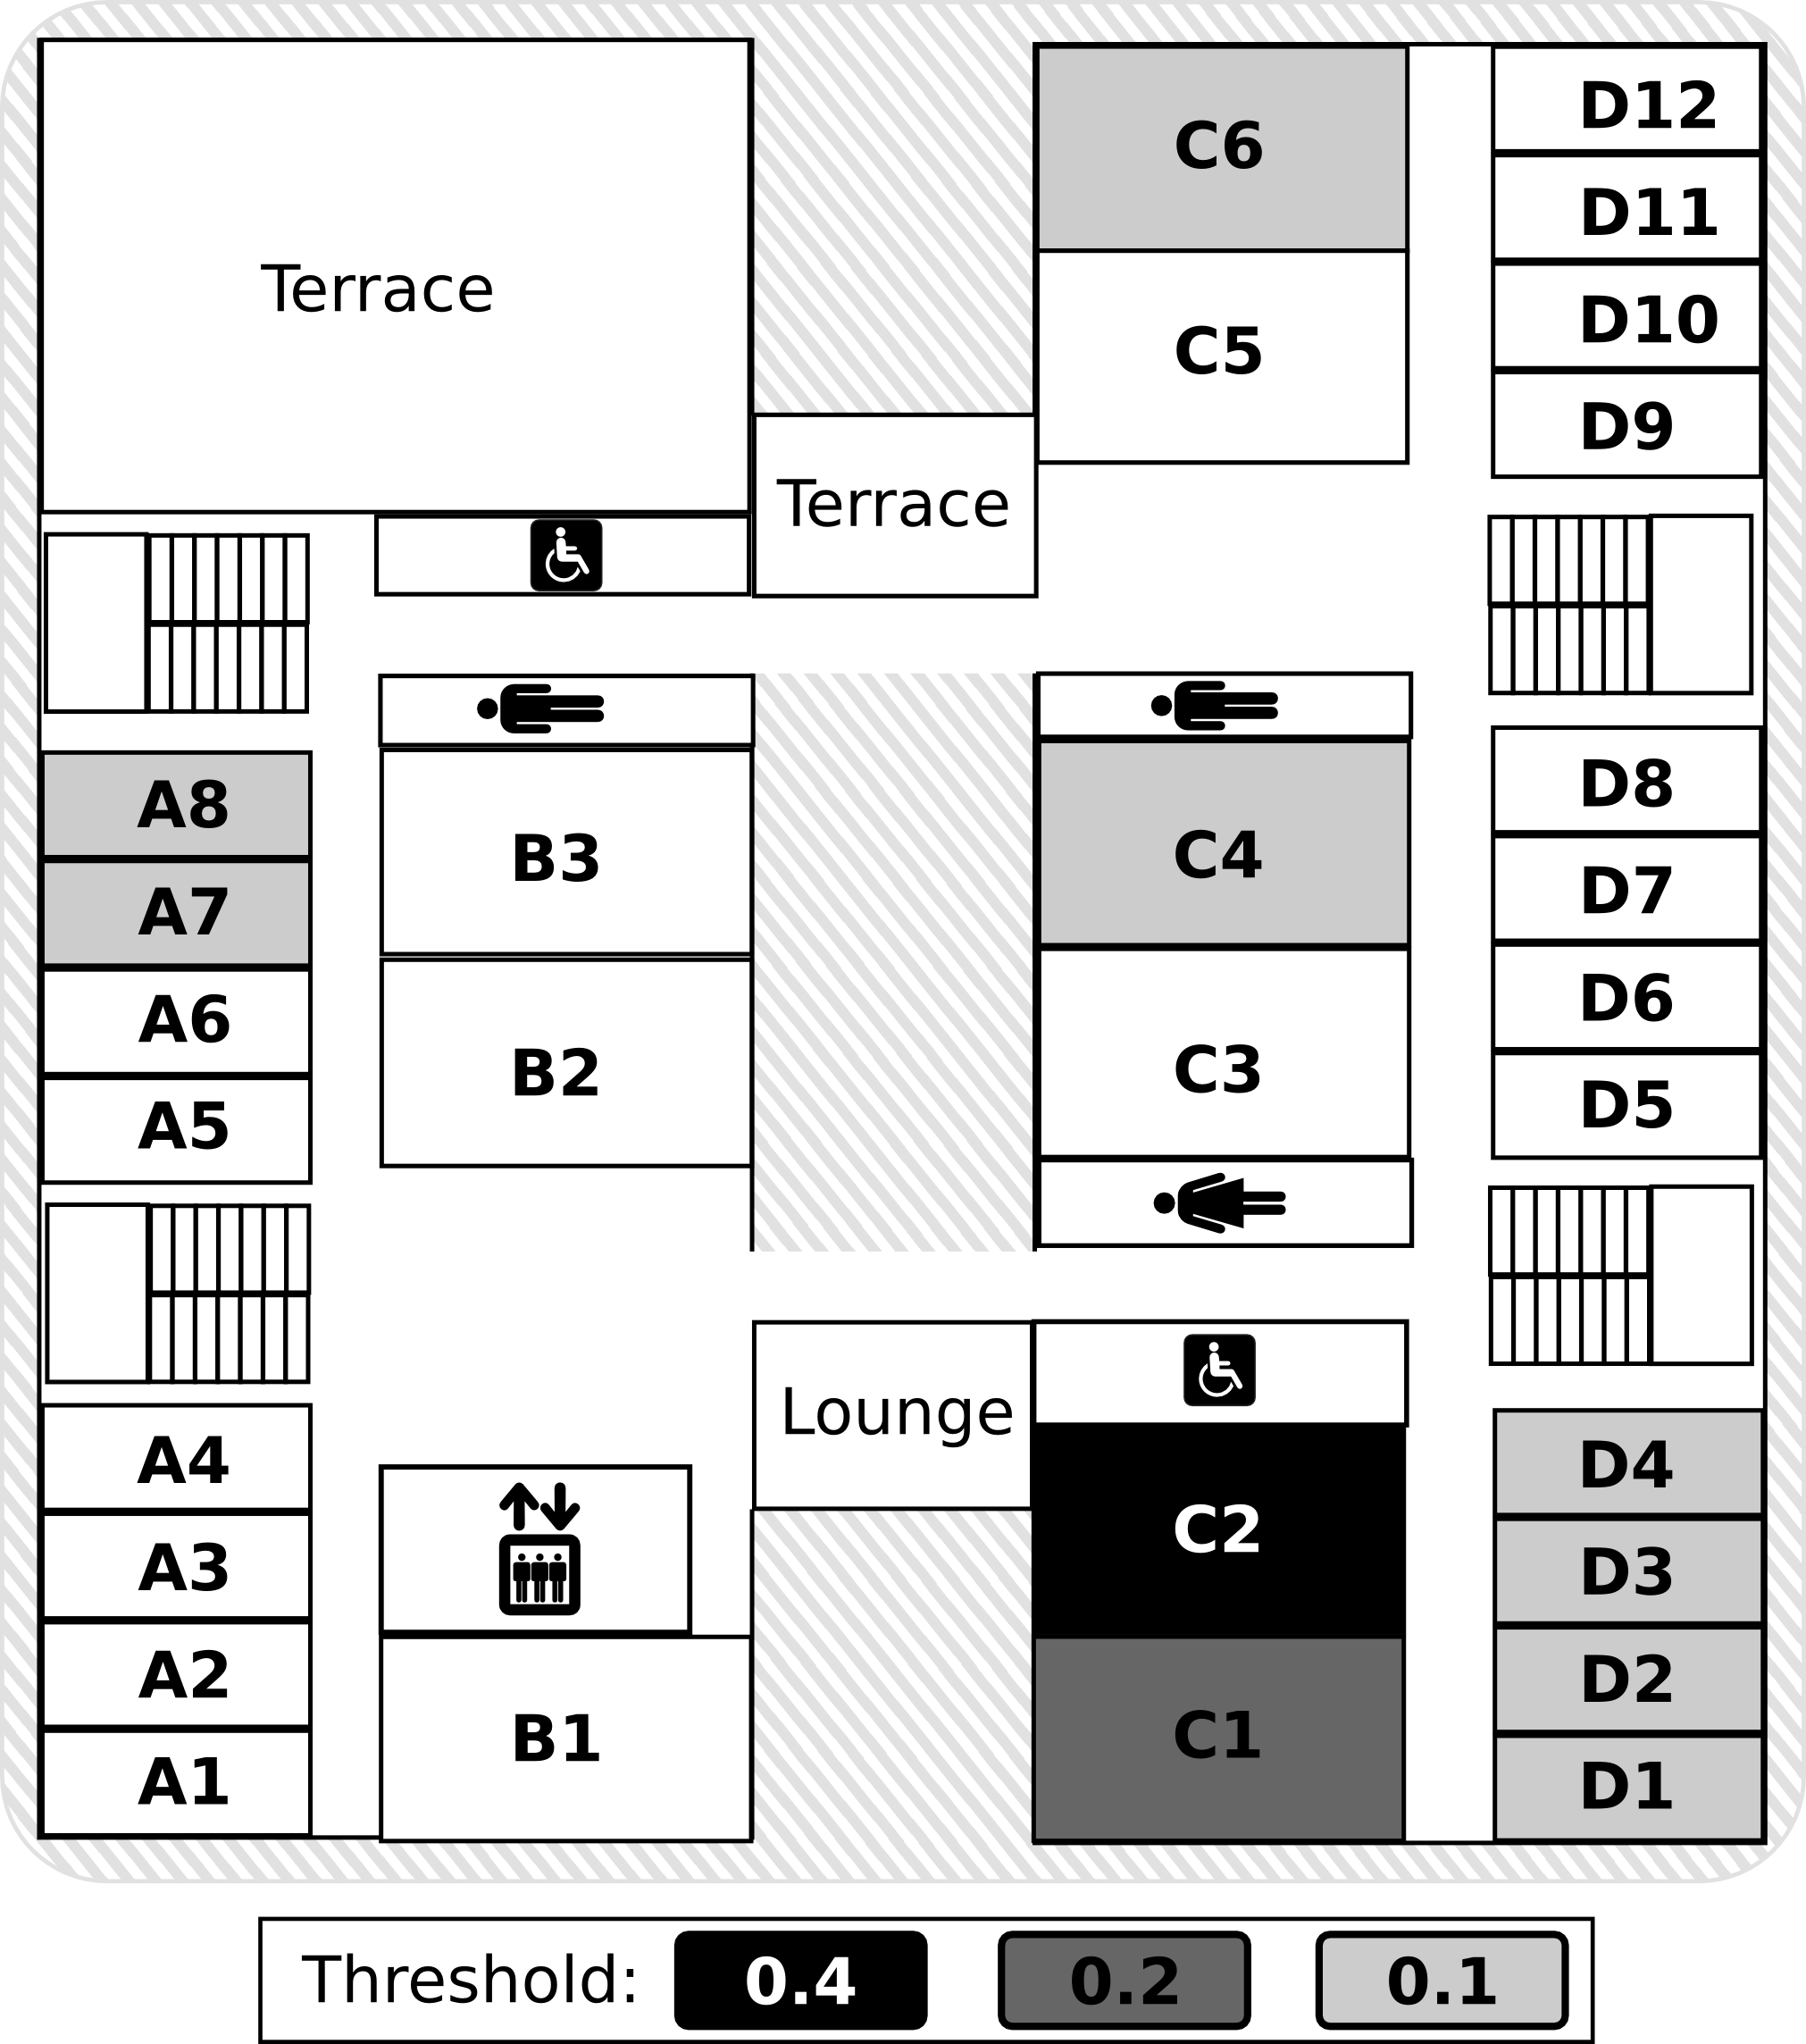
\includegraphics[width=.45\textwidth]{figs/floorMap.png}
\caption{Map of the floor where the analyzed EHP serves (room $C2$). The location of the sensors identified as related by the proposed approach are highlighted, showing a direct relationship between IMF correlation and spatial proximity.}
\label{fig:map}
\end{figure}

Figure \ref{fig:histo1} shows the distribution correlation coefficients.  Notice
that a large fraction of the dataset is correlated with the EHP trace.
\emph{Half} the traces have a correlation coefficient higher than $0.36$.  As expected, the underlying
trend is shared by a large number of device.
Although the highest score (i.e. $0.7715$) corresponds to the light in the same room that the EHP serves,
there are 118 pumps, serving all areas of the building, with a correlation higher than $0.6$.
Using only these results, it is not clear where the threshold should be set.  The distribution is close to 
uniform, making it difficult to 
know of how well your threshold discriminates against unrelated traces.
% Moreover, the distribution of the traces is almost uniform, thus, discriminating correlated traces is a laborious task.

Figure \ref{fig:histo2} shows the distribution of the average correlation value for the IMFs of
each trace and the EHP.  The number of traces correlated in the high frequency IMFs is significantly smaller
than the previous results. It's clear from the distribution that only a small set of devices are
\emph{intrinsically correlated} with the EHP.  In fact, \emph{only 10 traces out of 674} yielded a score higher than 
$0.25$. This allows us to easily rank traces by correlation.

Upon closer inspection of the 10 most correlated IMF traces, we find that there is a spatial relationship
between the EHP and the ten devices.  In fact, there is a direct relationship between score and distance from
the areas served by the EHP.  Figure~\ref{fig:map} shows a map of the floor that contains the rooms served by this
EHP.  The EHP directly serves room $C2$.  We introduce a correlation threshold to cluster correlated traces by score.
We highlight rooms by the threshold setting on the IMF correlation score.
When we set the threshold at $0.5$ we see that the sensors that have a correlation higher fall within room $C2$ --
the room served directly by the EHP.  As we relax the threshold, lowering it to $0.25$ and $0.1$ we see radial expansion from $C2$.  The trace with the highest score, $0.522$, is the trace corresponding to the lighting system \emph{in
the same room}.
The two highest scores for this floor (i.e. $0.316$ and $0.279$) are the light and EHP traces from next door, room $C1$.
Lower values correspond to sensors measuring activities in other rooms that have no specific relationship to the analyzed trace.  The results show a direct relationship between IMF correlation and spatial proximity and \emph{supports our initial
hypothesis}.


% Interestingly, the IMFs correlation coefficients reveal the spatial correlation of the sensors.
% Figure \ref{fig:map} is the map floor where the EHP trace is measured.
% Specifically, the EHP reports heating activity in the room $C2$.
% in the simple scenario the GHP is located in the room A5.



%\subsection{Limitations}
EMD is useful for finding underlying behavioral relationships between traces of sensor data.  However,
when we set the timescales smaller than a day, the results were not as strong.
The trace has to be long enough to capture the trend.  For this data set, the underlying
trend is daily, therefore it requires there to be a significant number of samples over many days.
%  to
% for this method to be effective.
Although this was a limitation for this dataset, it really depends on the underlying phenomenon that
the sensors are measuring.  Its underlying trend is ultimately what EMD will be able to separate
from the intrinsic modes of the underlying signal.

\subsection{Discussion}
EMD allows us to effectively identify fundamental relationships between sensor traces.
% Using EMD to find fundamental relationships between sensor traces effectively identifies intrinsically
% related behavioral relationships.
% was quite promising for building
% up models of correlated usage.  
We believe that identifying meaningful usage-correlation patterns can help reduce oversights
by the occupants and faults that lead to energy waste.  A direct application of this is the identification
of simultaneous heating and cooling~\cite{simheatcool}.  Simultaneous heating and cooling is when heating
and cooling system either compete with one another or compete with the incoming air from outside and is
a cause for major energy waste in building~\cite{simheatcool}.  The longer it goes undetected,
the more waste there is.  However, it is very difficult to identify since the occupants do not notice
changes in temperature.  Our analysis can be used to build a correlation model between the outside
heating cooling temperature, the cooling coil temperature, and the outside air vent position.  If their behavior
is not correlated as expect, an alarm should be raised.

We can also apply it to other usage scenarios.  In our traces, for example, we found an instance where the pump
was on, but the lights were off.  The two are typically correlated, however, in this case they were not.
The air conditioning was pumping cool air into a room without occupants.
With our approach this could have been identified and corrected.  In future work, we intend to
package our solution to serve these kinds of applications.

% EMD works perfectly although the weekly pattern of the data is altered the last analyzed week.

% EMD inherently finds the interesting time scales.

% number of zero crossing = mean frequency/time scale:
%   TODO give the time scale for each IMF.


\section{Conclusion}
% what is our problem

% what we did

% contributions and main results

% future work


This paper set out to examine the underlying relationship between sensor traces to find interesting correlations
in use.  We used data from a large deployment of sensors in a building and found that direct correlation analysis on the raw
traces was not discriminatory enough to find interesting relationships.  Upon closer inspection, we noticed that
the underlying trend was dominating the correlation calculation.  In order to extract meaningful behavior this trend has
to be removed.  We concluded that empirical mode decomposition is a helpful analytical tool for de-trending 
non-linear, non-stationary data; inherent attributes contained by our traces.

We re-ran our analysis on the same traces, except we correlated the IMF outputs of the EMD operation on each of the traces and found that the pump was closely related to the lights in the same room served by the pump and
uncorrelated with a pump on the same floor serving a different room.  In order to corroborate the applicability
of our approach, we compared the pump trace with \emph{all} 674 sensor traces and found a strong correlation
between the relative spatial position of the sensors and their IMF correlations.  The most correlated IMFs were 
serving the same
area in the building.  As we relax the admittance criteria we find that the spatial correlation expands radially from
the main location served by the reference trace.

We plan to examine the use of this method in applications that help discovery changes in underlying relationships over time
in order to identify opportunities for savings in buildings.  We will use it to build inter-device correlation models
and use these models to establish ``normal'', ``abnormal'' usage patterns.  We hope to take it a step further and include a
supervised learning approach to distinguish between ``efficient'' and ``inefficient'' usage patterns as well.








\vspace{+0.5mm}
\vspace{+2mm}
\bibliographystyle{abbrv}
%\scriptsize
\bibliography{references}
%\bibliography{references}

\end{document}


